\documentclass[border=0.2cm, 10pt]{standalone}
\usepackage{amsmath, amssymb}
\usepackage{tikz, pgfplots}
\pgfplotsset{compat=newest}
\usetikzlibrary{shapes, snakes, angles, quotes, arrows.meta}

\begin{document}

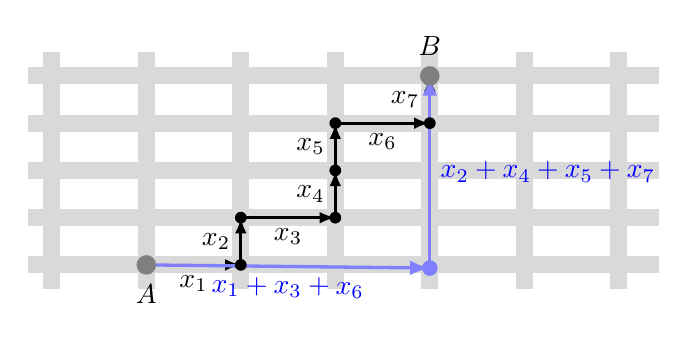
\begin{tikzpicture}[
    scale=1,
    line/.style={draw=gray!30, fill=gray!30},
    point/.style={fill=black, circle, inner sep=1.5pt},
    arrow/.style={-{Latex[length=2mm]}, line width=1.0pt, black},
    bluearrow/.style={-{Latex[length=2.5mm]}, line width=1.2pt, blue!50},
    endpoint/.style={fill=gray, circle, inner sep=2.5pt}
]

% Draw horizontal lines using a loop
\foreach \y in {0,0.6,1.2,1.8,2.4} {
    \draw[line] (0,\y) rectangle ++(8,0.2);
}

% Draw vertical lines using a loop
\foreach \x in {0.2,1.4,2.6,3.8,5,6.2,7.4} {
    \draw[line] (\x,-0.2) rectangle ++(0.2,3);
}

% Define coordinates for the path points
\coordinate (A) at (1.5,0.1);
\coordinate (B) at (2.7,0.1);
\coordinate (C) at (2.7,0.7);
\coordinate (D) at (3.9,0.7);
\coordinate (E) at (3.9,1.3);
\coordinate (F) at (3.9,1.9);
\coordinate (G) at (5.1,1.9);
\coordinate (H) at (5.1,2.5);

% Draw the black path with arrows
\draw[arrow] (A) -- node[below, sloped] {$x_1$} (B);
\draw[arrow] (B) -- node[left] {$x_2$} (C);
\draw[arrow] (C) -- node[below, sloped] {$x_3$} (D);
\draw[arrow] (D) -- node[left] {$x_4$} (E);
\draw[arrow] (E) -- node[left] {$x_5$} (F);
\draw[arrow] (F) -- node[below, sloped] {$x_6$} (G);
\draw[arrow] (G) -- node[left] {$x_7$} (H);

% Draw the blue path
\draw[bluearrow] (A) -- node[below, sloped, blue] {$x_1+x_3+x_6$} (5.1,0.06);
\draw[bluearrow] (5.1,0.06) -- node[right, pos=0.5, blue] {$x_2+x_4+x_5+x_7$} (H);

% Add points at each turn
\foreach \p in {B,C,D,E,F,G} {
    \node[point] at (\p) {};
}

% Add endpoints
\node[endpoint, label=below:{$A$}] at (A) {};
\node[endpoint, label=above:{$B$}] at (H) {};

% Add blue endpoint
\node[blue!50, circle, fill, inner sep=2pt] at (5.1,0.06) {};

\end{tikzpicture}

\end{document}
